\documentclass[a4paper, 12pt]{article}
\usepackage[utf8]{inputenc}
\usepackage[english, ukrainian]{babel}

\usepackage{amsmath, amssymb}
\usepackage{multicol}
\usepackage{graphicx}
\usepackage{float}

\allowdisplaybreaks
\setlength\parindent{0pt}
\numberwithin{equation}{subsection}

\usepackage{hyperref}
\hypersetup{unicode=true,colorlinks=true,linktoc=all,linkcolor=red}

\numberwithin{equation}{subsection}

\renewcommand{\bf}[1]{\textbf{#1}}
\renewcommand{\it}[1]{\textit{#1}}
\newcommand{\bb}[1]{\mathbb{#1}}
\renewcommand{\cal}[1]{\mathcal{#1}}

\renewcommand{\epsilon}{\varepsilon}
\renewcommand{\phi}{\varphi}

\DeclareMathOperator{\diam}{diam}
\DeclareMathOperator{\rang}{rang}
\DeclareMathOperator{\const}{const}

\newenvironment{system}{%
  \begin{equation}%
    \left\{%
      \begin{aligned}%
}{%
      \end{aligned}%
    \right.%
  \end{equation}%
}
\newenvironment{system*}{%
  \begin{equation*}%
    \left\{%
      \begin{aligned}%
}{%
      \end{aligned}%
    \right.%
  \end{equation*}%
}

\makeatletter
\newcommand*{\relrelbarsep}{.386ex}
\newcommand*{\relrelbar}{%
  \mathrel{%
    \mathpalette\@relrelbar\relrelbarsep%
  }%
}
\newcommand*{\@relrelbar}[2]{%
  \raise#2\hbox to 0pt{$\m@th#1\relbar$\hss}%
  \lower#2\hbox{$\m@th#1\relbar$}%
}
\providecommand*{\rightrightarrowsfill@}{%
  \arrowfill@\relrelbar\relrelbar\rightrightarrows%
}
\providecommand*{\leftleftarrowsfill@}{%
  \arrowfill@\leftleftarrows\relrelbar\relrelbar%
}
\providecommand*{\xrightrightarrows}[2][]{%
  \ext@arrow 0359\rightrightarrowsfill@{#1}{#2}%
}
\providecommand*{\xleftleftarrows}[2][]{%
  \ext@arrow 3095\leftleftarrowsfill@{#1}{#2}%
}
\makeatother

\newcommand{\NN}{\mathbb{N}}
\newcommand{\ZZ}{\mathbb{Z}}
\newcommand{\QQ}{\mathbb{Q}}
\newcommand{\RR}{\mathbb{R}}
\newcommand{\CC}{\mathbb{C}}

\newcommand{\Max}{\displaystyle\max\limits}
\newcommand{\Sup}{\displaystyle\sup\limits}
\newcommand{\Sum}{\displaystyle\sum\limits}
\newcommand{\Int}{\displaystyle\int\limits}
\newcommand{\Iint}{\displaystyle\iint\limits}
\newcommand{\Lim}{\displaystyle\lim\limits}

\newcommand*\diff{\mathop{}\!\mathrm{d}}

\newcommand*\rfrac[2]{{}^{#1}\!/_{\!#2}}


\title{{\Huge МАТЕМАТИЧНА ФІЗИКА}}
\author{Скибицький Нікіта}
\date{\today}

\usepackage{amsthm}
\usepackage[dvipsnames]{xcolor}
\usepackage{thmtools}
\usepackage[framemethod=TikZ]{mdframed}

\theoremstyle{definition}
\mdfdefinestyle{mdbluebox}{%
	roundcorner = 10pt,
	linewidth=1pt,
	skipabove=12pt,
	innerbottommargin=9pt,
	skipbelow=2pt,
	nobreak=true,
	linecolor=blue,
	backgroundcolor=TealBlue!5,
}
\declaretheoremstyle[
	headfont=\sffamily\bfseries\color{MidnightBlue},
	mdframed={style=mdbluebox},
	headpunct={\\[3pt]},
	postheadspace={0pt}
]{thmbluebox}

\mdfdefinestyle{mdredbox}{%
	linewidth=0.5pt,
	skipabove=12pt,
	frametitleaboveskip=5pt,
	frametitlebelowskip=0pt,
	skipbelow=2pt,
	frametitlefont=\bfseries,
	innertopmargin=4pt,
	innerbottommargin=8pt,
	nobreak=true,
	linecolor=RawSienna,
	backgroundcolor=Salmon!5,
}
\declaretheoremstyle[
	headfont=\bfseries\color{RawSienna},
	mdframed={style=mdredbox},
	headpunct={\\[3pt]},
	postheadspace={0pt},
]{thmredbox}

\declaretheorem[style=thmbluebox,name=Теорема,numberwithin=subsubsection]{theorem}
\declaretheorem[style=thmbluebox,name=Лема,numberwithin=subsubsection]{lemma}
\declaretheorem[style=thmbluebox,name=Твердження,numberwithin=subsubsection]{proposition}
\declaretheorem[style=thmbluebox,name=Принцип,numberwithin=subsubsection]{th_principle}
\declaretheorem[style=thmbluebox,name=Закон,numberwithin=subsubsection]{law}
\declaretheorem[style=thmbluebox,name=Закон,numbered=no]{law*}
\declaretheorem[style=thmbluebox,name=Формула,numberwithin=subsubsection]{th_formula}
\declaretheorem[style=thmbluebox,name=Рівняння,numberwithin=subsubsection]{th_equation}
\declaretheorem[style=thmbluebox,name=Умова,numberwithin=subsubsection]{th_condition}
\declaretheorem[style=thmbluebox,name=Наслідок,numberwithin=subsubsection]{corollary}

\declaretheorem[style=thmredbox,name=Приклад,numberwithin=subsubsection]{example}
\declaretheorem[style=thmredbox,name=Приклади,sibling=example]{examples}

\declaretheorem[style=thmredbox,name=Властивість,numberwithin=subsubsection]{property}
\declaretheorem[style=thmredbox,name=Властивості,sibling=property]{properties}

\mdfdefinestyle{mdgreenbox}{%
	skipabove=8pt,
	linewidth=2pt,
	rightline=false,
	leftline=true,
	topline=false,
	bottomline=false,
	linecolor=ForestGreen,
	backgroundcolor=ForestGreen!5,
}
\declaretheoremstyle[
	headfont=\bfseries\sffamily\color{ForestGreen!70!black},
	bodyfont=\normalfont,
	spaceabove=2pt,
	spacebelow=1pt,
	mdframed={style=mdgreenbox},
	headpunct={ --- },
]{thmgreenbox}

\mdfdefinestyle{mdblackbox}{%
	skipabove=8pt,
	linewidth=3pt,
	rightline=false,
	leftline=true,
	topline=false,
	bottomline=false,
	linecolor=black,
	backgroundcolor=RedViolet!5!gray!5,
}
\declaretheoremstyle[
	headfont=\bfseries,
	bodyfont=\normalfont\small,
	spaceabove=0pt,
	spacebelow=0pt,
	mdframed={style=mdblackbox}
]{thmblackbox}

\declaretheorem[name=Вправа,numberwithin=subsubsection,style=thmblackbox]{exercise}
\declaretheorem[name=Зауваження,numberwithin=subsubsection,style=thmgreenbox]{remark}
\declaretheorem[name=Визначення,numberwithin=subsubsection,style=thmblackbox]{definition}

\newtheorem{problem}{Задача}[subsection]
\newtheorem{sproblem}[problem]{Задача}
\newtheorem{dproblem}[problem]{Задача}
\renewcommand{\thesproblem}{\theproblem$^{\star}$}
\renewcommand{\thedproblem}{\theproblem$^{\dagger}$}
\newcommand{\listhack}{$\empty$\vspace{-2em}} 

\theoremstyle{remark}
\newtheorem*{solution}{Розв'язок}


\begin{document}
\tableofcontents

\setcounter{section}{2}

\section{Побудова математичних моделей базових фізичних процесів}

\setcounter{subsection}{-1}
\subsection{Оператор \texorpdfstring{$\nabla$}{nabla} (лікбез математичної теорії поля)}

\begin{definition}[оператора $\nabla$ в $\RR^2$]
    Для двовимірного евклідового простору $\RR^2$ у прямокутній декартовій системі координат \it{оператор набла} визначається наступним чином:
    \begin{equation}
    	\nabla = \frac{\partial}{\partial x} \vec{i} + \frac{\partial}{\partial y} \vec{j}
    \end{equation}
    де $\vec{i}$, $\vec{j}$ --- одиничні вектори по вісям $x$ і $y$ відповідно.
\end{definition}

\begin{definition}[оператора $\nabla$ в $\RR^3$]
    \begin{equation}
    	\nabla = \frac{\partial}{\partial x} \vec{i} + \frac{\partial}{\partial y} \vec{j} + \frac{\partial}{\partial z} \vec{k},
    \end{equation}
    де $\vec{i}$, $\vec{j}$, $\vec{k}$ --- одиничні вектори по вісям $x$, $y$ і $z$ відповідно.
\end{definition}

\subsubsection{Властивості оператора \texorpdfstring{$\nabla$}{nabla}}

\begin{definition}[градієнту через оператор $\nabla$]
	Якщо ``скалярно помножити'' вектор $\nabla$ на скалярну функцію $f = f(x, y, z)$, то вийде вектор:
	\begin{equation}
    	\nabla f = \frac{\partial f}{\partial x} \vec{i} + \frac{\partial f}{\partial y} \vec{j} + \frac{\partial f}{\partial z} \vec{k} = \left( \frac{\partial f}{\partial x}, \frac{\partial f}{\partial y}, \frac{\partial f}{\partial z} \right) = \grad f,
    \end{equation}
    який є нічим іншим як \it{градієнтом} $\grad f$ функції $f$.
\end{definition}

\begin{definition}[дивергенції через оператор $\nabla$]
	Якщо ``скалярно помножити'' вектор $\nabla$ на вектор-функцію
	\begin{equation}
	    \vec{F} = (f, g, h) = (f(x, y, z), g(x, y, z), h(x, y, z)),
	\end{equation}
	то вийде скаляр:
	\begin{equation}
    	\nabla \cdot \vec{F} = \frac{\partial f}{\partial x} + \frac{\partial g}{\partial y} + \frac{\partial h}{\partial z} = {\bf div} \vec{F},
    \end{equation}
    який є нічим іншим як \it{дивергенцією} $\divergence \vec{F}$ функції $\vec{F}$.
\end{definition}

\begin{definition}[ротора через оператор $\nabla$]
	Якщо ``векторно помножити'' вектор $\nabla$ на вектор-функцію
	\begin{equation}
	    \vec{F} = (f, g, h) = (f(x, y, z), g(x, y, z), h(x, y, z)),
	\end{equation}
	то вийде вектор:
	\begin{equation}
    	\begin{aligned}
        	\nabla \times \vec{F} &= \begin{vmatrix}
        		\vec{i} & \vec{j} & \vec{k} \\
        		\frac{\partial}{\partial x} & \frac{\partial}{\partial y} & \frac{\partial}{\partial z} \\
        		f & g & h
    		\end{vmatrix} = \\
    		&= \left( \frac{\partial h}{\partial y} - \frac{\partial g}{\partial z} \right) \vec{i} + \left( \frac{\partial f}{\partial z} - \frac{\partial h}{\partial x} \right) \vec{j} + \left( \frac{\partial g}{\partial x} - \frac{\partial f}{\partial y} \right) \vec{k} = \rot \vec{F}.
    	\end{aligned}
    \end{equation}
    який є нічим іншим як \it{ротором} $\rot \vec{F}$ функції $\vec{F}$.
\end{definition}

\begin{definition}[оператора Лапласа через оператор $\nabla$]
	Склаярний добуток $\nabla \cdot \nabla = \nabla^2$ є ніщо янше як оператор Лапласа, який також позначається $\Delta$. \medskip

	У декартових координатах оператор Лапласа має вигляд
	\begin{equation}
    	\Delta = \frac{\partial^2}{\partial x^2} + \frac{\partial^2}{\partial y^2} + \frac{\partial^2}{\partial z^2}.
    \end{equation}
\end{definition}

\subsubsection{Оператори другого порядку}

Оскільки існують різні способи множення веткорів і скалярів, з допомогою оператор набла можна записати різі види ``диференціювання''. так, комбінування склаярних і векторних добутків дає 7 різних варіантів ``похідних'' другого порядку:

\begin{align}
	& \divergence (\grad f) = \nabla \cdot (\nabla f) \\
	& \rot (\grad f) = \nabla \times (\nabla f) \\
	& \Delta f = \nabla^2 f) \\
	& \grad (\divergence \vec{F}) = \nabla (\nabla \cdot \vec{F}) \\
	& \divergence (\rot \vec{F}) = \nabla \cdot (\nabla \times \vec{F}) \\
	& \rot (\rot \vec{F}) = \nabla \times (\nabla \times \vec{F}) \\
	& \Delta \vec{F} = \nabla^2 \vec{F}
\end{align}

Для достатньо гладких полів (двічі неперервно диференційовних) ці оператори не незалежні. Два з них тотожньо дорівнюють нулю:

\begin{gather}
	\rot (\grad f) = \nabla \times (\nabla f) = (\nabla \times \nabla) f = 0 \\
	\divergence (\rot \vec{F}) = \nabla \cdot (\nabla \times \vec{F}) = (\nabla \times \nabla) \cdot \vec{F} = 0.
\end{gather}

Два завжди рівні:

\begin{equation}
	\divergence (\grad f) = \nabla \cdot (\nabla f) = (\nabla \cdot \nabla) f = \nabla^2 f = \Delta f.
\end{equation}

А решта три пов'язані співвідношенням:

\begin{equation}
	\nabla \times (\nabla \vec {F})= \nabla (\nabla \cdot \vec{F}) - \nabla^2 \vec{F}.
\end{equation}

І ще один може бути виражене через тензорний добуток векторів:

\begin{equation}
	\nabla (\nabla \cdot \vec{F}) = \nabla \cdot (\nabla \otimes \vec {F})
\end{equation}

\subsubsection{Приклади}

\begin{example}
	Нехай $z = z(x, y) = x y$, тоді
	\begin{equation}
		\nabla z = \frac{\partial z}{\partial x} \vec{i} + \frac{\partial z}{\partial y} \vec{j} = y \vec{i} + x \vec{j}.
	\end{equation}
\end{example}

\begin{example}
	Нехай $z = z(x, y) = 30 y x^3$, тоді
	\begin{equation}
		\nabla z = \frac{\partial z}{\partial x} \vec{i} + \frac{\partial z}{\partial y} \vec{j} = 90 y x^2 \vec{i} + 30 x^3 \vec{j}.
	\end{equation}
\end{example}

\subsection{Математичні моделі розповсюдження тепла та дифузії речовини}

Для запису математичної моделі введемо величини:
\begin{itemize}
	\item $x = (x_1, x_2, x_3) \in G \subset \RR^3$ об'єм тіла, $t$ --- час;
	\item $u(x, t)$ --- температура в точці $x$ у момент часу $t$;
	\item $c(x)$ --- теплоємність (кількість тепла, яка необхідна, для підняти температуру одиниці маси тіла на один градус);
	\item $k(x)$ --- теплопровідність речовини (здатність проводити тепло);
	\item $\rho(x)$ --- щільність речовини;
	\item $f(x, t)$ --- інтенсивність джерел теплової енергії в точці $x$ в момент часу $t$.
\end{itemize}

\subsubsection{Закон збереження теплової енергії}

Складемо баланс теплової енергії для довільного об'єму тіла $G$ за довільний інтервал часу $t_1 < t < t_2$. Для цього обчислимо кількість тепла, яка міститься в нескінченно малому об'ємі $\diff G$: 
\begin{equation}
	\rho(x) \cdot \diff G \cdot c(x) \cdot u(x, t)
\end{equation}
та в об'ємі $G$ в момент часу $t$:
\begin{equation}
	Q_1(t) = \Iiint_G c(x) \rho(x) u(x, t) \diff G.
\end{equation}

Припустимо, що з часом температура змінилася від значення $u(x, t_1)$ до значення $u(x, t_2)$. Обчислимо кількість тепла, витрачену на зміну температури:
\begin{equation}
	\Delta Q_1(t_1, t_2) = Q_1(t_2) - Q_1(t_1) = \Iiint_G c(x) \rho(x) (u(x, t_2) - u(x, t_1)) \diff G.
\end{equation}

Температура в об'ємі $G$ може змінюватись за рахунок таких факторів:
\begin{enumerate}
	\item нерівномірності нагрівання тіла, викликає потік тепла через поверхню $S$, яка обмежує уявне тіло об'єму $G$;
	\item зміна кількості тепла за рахунок внутрішніх теплових джерел.
\end{enumerate}

Нехай $\vec n$ --- зовнішня нормаль до поверхні $S$. Обчислимо кількість тепла, яка поступає всередину об'єму $G$ через елементарну поверхню $\diff S$ в одиницю часу: 
\begin{equation}
	\diff Q(x, t) = k(x) \cdot \frac{\partial u(x, t)}{\partial \vec n} \cdot \diff S
\end{equation}

Ця формула є математичним виразом фізичного закону Фур'є. \medskip

Кількість тепла, яка проходить через всю поверхню $S$ за час від $t_1$ до $t_2$ обчислюється за формулою
\begin{equation}
	Q_2(t_1, t_2) = \Int_{t_1}^{t_2} \Iint_S \left( k(x) \cdot \frac{\partial u(x, t)}{\partial \vec n} \right) \diff S \diff t.
\end{equation}

Кількість тепла за рахунок теплових джерел в об'ємі $G$ можна обчислити у вигляді:
\begin{equation}
	Q_3(t_1, t_2) = \Int_{t_1}^{t_2} \Iiint_G f(x, t) \diff G \diff t.
\end{equation}

Таким чином можна записати 
\begin{law*}[збереження теплової енергії]
	Виконується співвідношення:
	\begin{equation}
		\Delta Q_1(t_1, t_2) = Q_2(t_1, t_2) + Q_3(t_1, t_2),
	\end{equation}
\end{law*}
або після підстановки усіх величин маємо 
\begin{law*}[збереження теплової енергії  в інтегральному вигляді]
	Виконується співвідношення:
	\begin{multline}
		\Iiint_G c(x) \rho(x) (u(x, t_2) - u(x, t_1)) \diff G = \\
		= \Int_{t_1}^{t_2} \Iint_S \left( k(x) \cdot \frac{\partial u(x, t)}{\partial \vec n} \right) \diff S \diff t + \Int_{t_1}^{t_2} \Iiint_G f(x, t) \diff G \diff t.
	\end{multline}
\end{law*}

Для перетворення першого інтегралу правої частини останньої рівності застосуємо формулу Остроградського Гауса, 
\begin{equation}
	\Iint_S \langle A, \vec n \rangle \diff S = \Iiint_G \Big(\nabla \cdot \vec A\Big) \diff G,
\end{equation}
де $\vec A$ --- векторне поле,
\begin{equation}
	\nabla \cdot A = \frac{\partial A_1}{\partial x_1} + \frac{\partial A_2}{\partial x_2} + \frac{\partial A_3}{\partial x_3}.
\end{equation}

В результаті отримаємо:
\begin{multline}
	\Int_{t_1}^{t_2} \Iiint_G \left( c(x)\rho(x) \frac{\partial u(x, t)}{\partial t} \right) \diff G \diff t = \\
	= \Int_{t_1}^{t_2} \Iiint_G \left( \nabla \cdot (k(x) \nabla u) \right) \diff G \diff t + \Int_{t_1}^{t_2} \Iiint_G f(x, t) \diff G \diff t.
\end{multline}

Враховуючи, що остання рівність отримана для довільного об'єму $G$ та довільних моментів часу, можна зробити висновок, що вона має місце тоді і лише тоді, коли має місце рівність підінтегральних виразів:
\begin{equation}
	\label{eq:thermal-energy-is-const}
	c(x) \rho(x) \frac{\partial u(x, t)}{\partial t} =\nabla\cdot (k(x) \nabla u) + f(x, t),
\end{equation}
де $x \in G$, $t > 0$. \medskip

Це рівняння повинно виконуватись для кожної точки $x$ реального фізичного об'єму тіла (збережемо для нього позначення $G$, а для його поверхні позначення $S$), та для кожного моменту часу $t$. \medskip

Для виділення єдиного розв'язку цього рівняння окрім самого диференціального рівняння необхідно задавати додаткові умови на границі просторово-часової області. Будемо використовувати фізичні міркування для задавання таких умов.

\begin{enumerate}
	\item Якщо на границі області відома температура тіла, тоді на границі тіла задають умову Діріхле.

	\begin{definition}[умови Діріхле]
		Крайовою умовою першого роду, або \it{умовою Діріхле} називають співвідношення
		\begin{equation}
			\left. u(x, t) \right|_{x \in S} = v(x, t).		 							
		\end{equation}
	\end{definition}

	\item Якщо на границі області відомий тепловий потік в одиницю часу, який поступає всередину тіла через одиничну площу, тоді на границі задають граничну умову Неймана.

	\begin{definition}[умови Неймана]
		Крайовою умовою другого роду, або \it{умовою Неймана} називають співвідношення
		\begin{equation}
			\left. k(x) \frac{\partial u(x, t)}{\partial \vec n} \right|_{x \in S} = q(x, t).
		\end{equation}
	\end{definition}

	\item Якщо на границі тіла відбувається конвективний теплообмін з оточуючим середовищем відомої температури згідно до закону Ньютона, тоді на границі задають крайову умову Ньютона
	\begin{definition}[умови Ньютона]
		Крайовою умовою третього роду, або \it{умовою Ньютона} називають співвідношення
		\begin{equation}
			\left. k(x) \frac{\partial u(x, t)}{\partial \vec n} \right|_{x \in S} = \left. \alpha(x, t) (v(x, t) - u(x, t)) \right|_{x \in S},
		\end{equation}
		де $\alpha(x, t) > 0$ --- коефіцієнт теплообміну, $v(x, t)$ --- температура оточуючого середовища.
	\end{definition}

	\item В початковий момент часу задають температура усіх внутрішніх точок тіла:
	\begin{equation}
		\left. u(x, t) \right|_{t = 0} = u_0(x).
	\end{equation}

	\begin{definition}[початкової умови]
		\it{Початковою умовою} називається співвідношення
		\begin{equation}
			\left. u(x, t) \right|_{t = 0} = u_0(x),
		\end{equation}
		при цьому $u_0(x)$ називається \it{початковою температурою}.
	\end{definition}
\end{enumerate}

\subsubsection{Частинні випадки рівняння теплопровідності}

\begin{remark}
	У випадку, коли коефіцієнт теплопровідності та інтенсивність теплових джерел залежить не лише від точки простору і часу, а і від самої температури, тобто $k = k(u, x, t)$, $f = f(u, x, t)$, лінійне диференціальне рівняння \eqref{eq:thermal-energy-is-const} стає квазілінійним, тобто лінійним відносно старших похідних.
\end{remark}

Окрім загального вигляду рівняння теплопровідності, у практичних випадках часто використовуються частинні випадки рівняння. \medskip

Зокрема, можна розглядати розповсюдження тепла в одновимірних та двовимірних тілах:
\begin{itemize}
	\item У пластині:
	\begin{equation}
		\nabla \cdot (k(x) \nabla u(x, t)) = \frac{\partial}{\partial x_1} \left( k(x) \frac{\partial u(x, t)}{\partial x_1} \right) + \frac{\partial}{\partial x_2} \left( k(x) \frac{\partial u(x, t)}{\partial x_2} \right).
	\end{equation}
	\item У стрижні:
	\begin{equation}
		\nabla \cdot (k(x) \nabla u(x, t)) = \frac{\partial}{\partial x} \left( k(x) \frac{\partial u(x, t)}{\partial x} \right).
	\end{equation}
\end{itemize}

Для однорідних тіл усі коефіцієнти рівняння можна вважати константами, зокрема $c = c_0$, $\rho = \rho_0$, $k = k_0$. В результаті вищезгадане диференціальне рівняння буде мати вигляд
\begin{equation}
	\frac{\partial u(x, t)}{\partial t} = a^2 \Delta u + \frac{1}{c_0 \rho_0} \cdot f(x, t),
\end{equation}
де 
\begin{equation}
	a^2 = \frac{k_0}{c_0 \rho_0} > 0,
\end{equation}
і було введено
\begin{definition}[оператор Лапласа]
	\it{Оператором Лапласа} називається диференціальний оператор $\Delta$ що діє на функцію $u(x, t)$ по векторній змінній $x$ наступним чином:
	\begin{equation}
		\Delta u(x, t) = \nabla \cdot (\nabla u(x, t)) = \Sum_{i = 1}^n \frac{\partial^2 u(x, t)}{\partial x_i^2}.
	\end{equation}
\end{definition}

\begin{remark}
	Зокрема одновимірне рівняння теплопровідності має вигляд:
	\begin{equation}
		\frac{\partial u(x, t)}{\partial t} = a^2 \frac{\partial^2 u(x, t)}{\partial x^2} + \frac{1}{c_0 \rho_0} f(x, t).
	\end{equation}
\end{remark}

\subsubsection{Рівняння дифузії речовини}

Процес дифузії речовини це процес вирівнювання концентрації речовини у розчинах, розплавах або в сумішах. Фізика вирівнювання температури в тілах та концентрації у розчинах чи розплавах має багато схожих рис і з цього приводу навіть процес розповсюдження тепла називають дифузією тепла. \medskip

Для отримання моделі дифузії речовини використаємо наступну таблицю аналогії.
\begin{table}[H]
	\centering
	\begin{tabular}{| C{3.75cm} | C{3.75cm} | L{4.5cm} |}
		\hline
		Дифузія & Теплопровідність & Пояснення \\ \hline
		$u(x, t)$ & $u(x, t)$ & Концентрація речовини в розчині, або у розплаві \\ \hline
		$c(x)$ & $c(x) \rho(x)$ & Коефіцієнт пористості, відображає відношення об'єму пор до загального об'єму тіла і вказує на кількість речовини необхідну для зміни концентрації на одну одиницю в одиниці об'єму. \\ \hline
	\end{tabular}
\end{table}

\begin{table}[H]
	\centering
	\begin{tabular}{| C{3.75cm} | C{3.75cm} | L{4.5cm} |}
		\hline
		Дифузія & Теплопровідність & Пояснення \\ \hline
		$D \dfrac{\partial u}{\partial \vec n} \diff S$ & $k \dfrac{\partial u}{\partial \vec n} \diff S$ & Закон Нерста, описує кількість речовини, яка поступає всередину тіла через його поверхню в одиницю часу за рахунок нерівномірності концентрації. \\ \hline
		$f(x, t)$ & $f(x, t)$ & Інтенсивність джерела речовини в середині об'єму. \\ \hline
 		$D \dfrac{\partial u}{\partial \vec n} = \alpha \left. (v - u)\right|_S$ & $k \dfrac{\partial u}{\partial \vec n} = \alpha \left. (v - u)\right|_S$ & Кількість речовини, яка поступає через поверхню $S$ тіла за законом, аналогічним закону Ньютона,
 		$v$ --- відома концентрація речовини в тому чи іншому середовищі; $\alpha$ --- коефіцієнт проникності поверхні. \\ \hline
 	\end{tabular}
\end{table}

Побудови математичної моделі процесу дифузії відбувається за аналогією згідно до попередньої таблиці. \medskip

Кількість речовини, яка витрачена для зміни концентрації від $u(x, t_1) \to u(x, t_2)$, $t_1 < t_2$ має вигляд:
\begin{equation}
	\Delta Q_1(t_1, t_2) = Q_1(t_2) - Q_1(t_1) = \Iiint_G c(x) (u(x, t_2) - u(x, t_1)) \diff G.
\end{equation}

Кількість речовини, яка проходить через всю поверхню $S$ за час від $t_1 \to t_2$:
\begin{equation}
	Q_2(t_1, t_2) = \Int_{t_1}^{t_2} \Iint_S \left( D(x, t) \frac{\partial u}{\partial \vec n} \right) \diff S \diff t.
\end{equation}

Кількість речовини, яка поступає за рахунок джерел речовини в об'ємі $G$ за час від $t_1$ до $t_2$:
\begin{equation}
	Q_3(t_1, t_2) = \Int_{t_1}^{t_2} \Iiint_G f(x, t) \diff G \diff t.
\end{equation}

Отже, отримали 
\begin{law*}[збереження маси]
	Вионується співвідношення:
	\begin{equation}
		\Delta Q_1(t_1, t_2) = Q_2(t_1, t_2) + Q_3(t_1, t_2).
	\end{equation}
\end{law*}
а також
\begin{law*}[збереження маси в інтегральному вигляді]
	Вионується співвідношення:
	\begin{multline}
		\Iiint_G c(x) (u(x, t_2) - u(x, t_1)) \diff G = \\
		= \Int_{t_1}^{t_2} \Iint_S \left( D(x, t) \frac{\partial u(x, t)}{\partial \vec n} \right) \diff S \diff t + \Int_{t_1}^{t_2} \Iiint_G f(x, t) \diff G \diff t.
	\end{multline}
\end{law*}

Після застосування формули Остроградського-Гауса та прирівнювання підінтегральних виразів отримаємо рівняння дифузії речовини у вигляді:
\begin{equation}
	c(x) \frac{\partial u}{\partial t} = \nabla \cdot (D(x, t) \nabla u) + f(x, t),
\end{equation}
де $x \in G$, $t > 0$. \medskip

Додаткові умови на границі області задають аналогічно умовам для рівняння теплопровідності:
\begin{enumerate}
	\item Якщо відома концентрація речовини на поверхні:
	\begin{equation}
		\left. u(x, t) \right|_{x \in S} = v(x, t);
	\end{equation}

	\item Якщо на границі відомий потік речовини:
	\begin{equation}
		\left. D \cdot \frac{\partial u(x, t)}{\partial \vec n} \right|_{x \in S} = g(x, t);
	\end{equation}

	\item Якщо на границі відбувається обмін речовиною з оточуючим середовищем через напівпроникливу мембрану за законом аналогічним закону Ньютона:
	\begin{equation}
		\left. D(x,t) \frac{\partial u(x, t)}{\partial \vec n} \right|_{x \in S} = \alpha(x,t) \left. ( v(x, t) - u(x, t) ) \right|_{x \in S};
	\end{equation}

	\item Якщо в початковий момент часу відома концентрація речовини:
	\begin{equation}
		u(x, 0) = u_0(x).
	\end{equation}
\end{enumerate}

\begin{remark}
	У випадку, коли коефіцієнти рівняння та граничних умов не залежать від часу $t$, розв'язок рівняння не залежить від часу в результаті отримаємо стаціонарне рівняння теплопровідності та дифузії:
	\begin{align}
		\nabla \cdot (k(x) \nabla u(x)) &= -f(x), \\
		\nabla \cdot (D(x) \nabla u(x)) &= -f(x).
	\end{align}
\end{remark}

\subsubsection{Задача Стефана (задача про остигання та затвердіння розплавленого металу)}

Вертикальний циліндричний посуд заповнений розплавленим металом, який знаходиться при заданій температурі $U_0 > U_{melt}$ - температура плавління металу. Починаючи з моменту часу $t_0$ вільна поверхня розплавленого металу підтримується при постійній температурі $U_1 < U_{melt}$. Поставимо задачу про остудження та затвердіння металу, якщо дно і бокова поверхня посуду теплоізольовані. Термічними деформаціями об'єму будемо нехтувати тобто процес розповсюдження тепла відбувається лише вздовж вісі циліндру. Введемо позначення: 
\begin{itemize}
 	\item $\rho_s$, $\rho_l$ --- щільність твердої (eng. \it{solid}) та рідкої (eng. \it{liquid}) фази металу;
	\item $c_s$, $c_l$ --- теплоємність твердої та рідкої фази металу;
	\item $k_s$, $k_l$ --- теплопровідність твердої та рідкої фази металу;
	\item $\xi(t)$ --- положення границі розділу твердої та рідкої фаз;
	\item $L$ --- висота циліндру, $S$ --- площа основи циліндру; 
	\item $\lambda$ --- питома теплота плавлення;
	\item $u(x, t)$ --- температура в момент часу $t$ в точці $x$.
\end{itemize}

Деякі з введених позначень краще видно на наступній ілюстрації:
\begin{figure}[H]
	\centering
	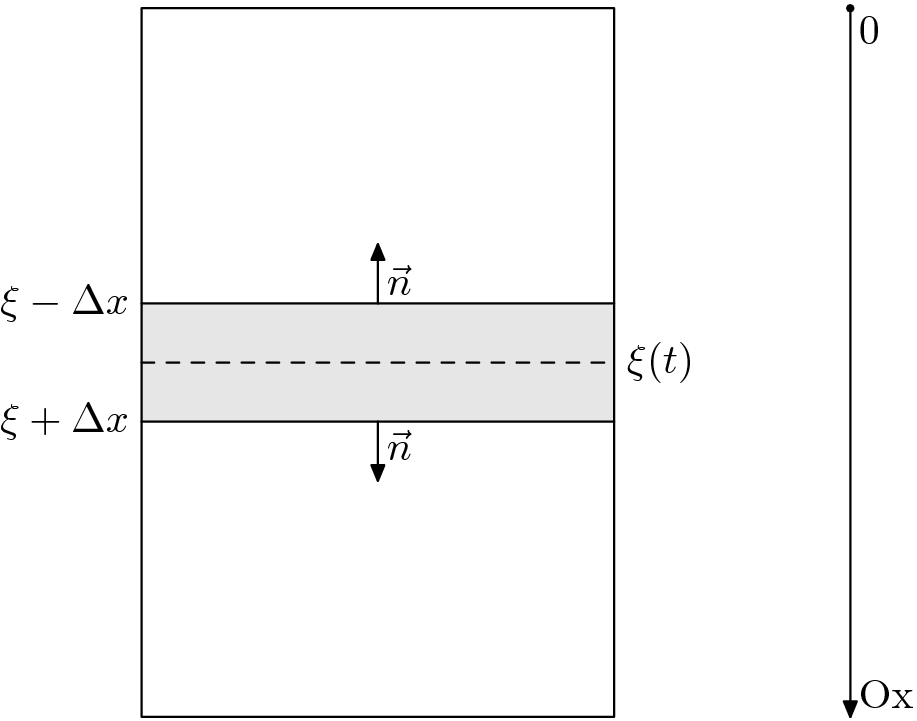
\includegraphics[width=.7\textwidth]{{../img/7-1}.mps}
\end{figure}

Отримаємо рівняння теплового балансу для нескінченно малого об'єму розплавленого металу, який знаходиться між перерізами $x$ та $x + \Delta x$ за проміжок часу від $t$ до $t + \Delta t$. \medskip

Обчислимо кількість тепла, яка необхідна для зміни температури у виділеному елементарному об'ємі від значення $u(x, t)$ до значення $u(x, t + \Delta t)$. Кількість тепла, що міститься в виділеному об'ємі в момент часу $t$ можна обчислити за формулою
\begin{equation}
	\diff Q(t) = c_l \cdot \rho_l \cdot S \cdot \Delta x \cdot u(x, t).
\end{equation}

Аналогічно для моменту часу $t + \Delta t$ кількість тепла дорівнює
\begin{equation}
	\diff Q(t + \Delta t) = c_l \cdot \rho_l \cdot S \cdot \Delta x \cdot u(x, t + \Delta t).
\end{equation}

При цьому нехтуємо, зміною температури по просторовій змінній у середині елементарного об'єму. Тоді кількість тепла, необхідна для зміни температури всередині об'єму дорівнює:
\begin{equation}
	\Delta Q(t, t + \Delta t) = c_l \cdot \rho_l \cdot S \cdot \Delta x \cdot (u(x, t + \Delta t) - u(x, t)).
\end{equation}

Ця зміна може відбуватися за рахунок теплових потоків, через перерізи $x$ та $x + \Delta x$. Підрахуємо кількість тепла, яка поступає всередину тіла через переріз $x + \Delta x$ за час $\Delta t$:
\begin{equation}
	\diff Q(x + \Delta x) = k_l \frac{\partial u(x + \Delta x, t)}{\partial \vec n} S \Delta t= k_l \frac{\partial u(x + \Delta x, t)}{\partial x} S \Delta t
\end{equation} 
 
Напрям нормалі $\vec n$ в цьому перерізі співпадає з напрямом вісі $Ox$. \medskip

Кількість тепла, яка поступає всередину тіла через переріз $x$ за час $\Delta t$ можна записати у вигляді:
\begin{equation}
	\diff Q(x) = k_l \frac{\partial u(x, t)}{\partial \vec n} S \Delta t = - k_l \frac{\partial u(x, t)}{\partial x} S \Delta t
\end{equation} 

Таким чином можна скласти рівняння теплового балансу:
\begin{equation}
	\diff Q(t, t + \Delta t) = \diff Q(x + \Delta x) + \diff Q(x).
\end{equation}
 
Або після підстановки відповідних значень поділених на $\Delta x \cdot \Delta t \cdot S$ отримаємо:
\begin{equation}
	\frac{c_l \rho_l (u(x, t + \Delta t) - u(x, t))}{\Delta t} = k_l \left( \frac{\partial u(x + \Delta x, t)}{\partial x} - \frac{\partial u(x, t)}{\partial x} \right) \frac{1}{\Delta x}.
\end{equation}
 
Після граничного переходу коли $\Delta x$ та $\Delta t$ прямують до нуля, отримаємо диференціальне рівняння:
\begin{equation}
	\label{eq:liquid-phase-diff-eq}
	c_l \rho_l \frac{\partial u(x, t)}{\partial t} = k_l \frac{\partial^2 u(x, t)}{\partial x^2},
\end{equation}
де $\xi(t) < x < L$, $t > t_0$. \medskip

Аналогічні міркування дозволяють отримати рівняння для твердої фази:
\begin{equation}
	\label{eq:solid-phase-diff-eq}
	c_s \rho_s \frac{\partial u(x, t)}{\partial t} = k_s \frac{\partial^2 u(x, t)}{\partial x^2},
\end{equation}
де $0 < x < \xi(t)$, $t > t_0$. \medskip

\begin{definition}[співвідношення на границі розділу фаз]
	Температура при переході через границю розділу фаз повинна змінюватись неперервно і співпадати з температурою плавлення металу, тобто повинно виконуватись настуну співвідношення:
	\begin{equation}
		\label{eq:phase-border-conditions}
		u(\xi(t) - 0, t) = u(\xi(t) + 0, t) = U_{melt},
	\end{equation}
	яке називається \it{співвідношенням на границі розділу фаз}.
\end{definition}

Отримаємо рівняння теплового балансу для елементарного об'єму обмеженого перерізами $\xi(t) - \Delta x$ та $\xi(t) + \Delta x$. \medskip

За час $\Delta t$ затвердіє об'єм металу рівний
\begin{equation}
	(\xi(t + \Delta t) - \xi(t)) \cdot S.
\end{equation}

При цьому буде виділено кількість тепла рівна
\begin{equation}
	\diff Q_{melt} = (\xi(t + \Delta t) - \xi(t)) \cdot S \cdot \lambda \cdot \rho_s.
\end{equation}

Кількість тепла, яка надійде всередину об'єму за рахунок теплових потоків через відповідні перерізи за час $\Delta t$ може бути записана у вигляді:
\begin{equation}
	\Delta t \cdot S \cdot \left( k_l \cdot \frac{\partial u(\xi(t) + \Delta x, t)}{\partial x} - k_s \cdot \frac{\partial u(\xi(t) - \Delta x, t)}{\partial x}\right).
\end{equation}
 
Оскільки фазовий перехід відбувається при постійній температурі, то в околі границі розділу фаз $\xi(t)$ зміною температури по змінній $t$ можна нехтувати, в зв'язку з чим можна не враховувати кількість тепла, яка витрачається на зміну температури у виділеному елементарному об'ємі. \medskip

Рівняння теплового балансу для елементарного об'єму обмеженого перерізами $\xi(t) - \Delta x$ та $\xi(t) + \Delta x$ можна записати у вигляді:
\begin{multline}
	(\xi(t + \Delta t) - \xi(t)) S \lambda \rho_s = \\
	= \Delta t S \left( k_l \frac{\partial u(\xi(t) + \Delta x, t)}{\partial x} - k_s \frac{\partial u(\xi(t) - \Delta x, t)}{\partial x}\right)
\end{multline}

Поділивши обидві частини на $\Delta t$, скоротивши на $S$ і спрямувавши $\Delta x$, $\Delta t$ до нуля отримаємо співвідношення:
\begin{equation}
	\lambda \rho_s \frac{\partial \xi(t)}{\partial t} = k_l \frac{\partial u(\xi(t) + 0, t)}{\partial x} - k_s \frac{\partial u(\xi(t) - 0, t)}{\partial x}.
\end{equation}

\begin{definition}[внутрішніх граничних умов (умов спряження)]
	Останню умову 
	\begin{equation}
		\label{eq:conjugate-conditions}
		\lambda \rho_s \frac{\partial \xi(t)}{\partial t} = k_l \frac{\partial u(\xi(t) + 0, t)}{\partial x} - k_s \frac{\partial u(\xi(t) - 0, t)}{\partial x}.
	\end{equation}
	разом із співвідношенням \eqref{eq:phase-border-conditions} на границі розділу фаз називають \it{внутрішніми граничними умовами}, або \it{умовами спряження}.
\end{definition}

Запишемо початкові умови та умови на верхній та нижній основі циліндру:
\begin{itemize}
	\item В початковий момент часу задана температура розплавленого металу:
	\begin{equation}
		\label{eq:start-time-temp}
		u(x, t_0) = U_0, \quad 0 < x < L.
	\end{equation}
	
	\item На верхній основі задана температура:
	\begin{equation}
		\label{eq:upper-cylinder-border-temp}
		u(0, t) = U_1, \quad t > t_0.
	\end{equation}

	\item Нижня основа теплоізольована, тобто тепловий потік, який поступає всередину тіла дорівнює нулю:
	\begin{equation}
		\label{eq:lower-cylinder-border-temp-flow}
		\frac{\partial u(L, t)}{\partial x} = 0, \quad t > t_0.
	\end{equation}
	
	\item В початковий момент часу положення границі фазового переходу співпадає з верхньою основою циліндру: 
	\begin{equation}
		\label{eq:start-time-xi}
		\xi(t_0) = 0.
	\end{equation}
\end{itemize}

Таким чином, до моменту часу, коли весь метал затвердіє постановка задачі Стефана включає в себе диференційні рівняння \eqref{eq:liquid-phase-diff-eq}, \eqref{eq:solid-phase-diff-eq}, співвідношення на границі розділу фаз \eqref{eq:phase-border-conditions}, умови спряження \eqref{eq:conjugate-conditions}, початкові умови \eqref{eq:start-time-temp}, \eqref{eq:start-time-xi} та граничні умови \eqref{eq:upper-cylinder-border-temp}, \eqref{eq:lower-cylinder-border-temp-flow}. \medskip

\begin{remark}
	Після повного затвердіння металу, тобто коли $\xi(t_1) = L$, процес буде описуватись звичайним рівнянням теплообміну для $t > t_1$ з граничними умовами
	\begin{align}
		u(0, t) &= U_1, \\
		\frac{\partial u(L, t)}{\partial x} &= 0,
	\end{align}
	та початковою температурою $u(x, t_1)$.
\end{remark}

\end{document}
